\documentclass[crop,class=article]{standalone}
%----------------------------Preamble-------------------------------%
\usepackage{tikz}             % Drawing/graphing tools.
%--------------------------Main Document----------------------------%
\begin{document}
    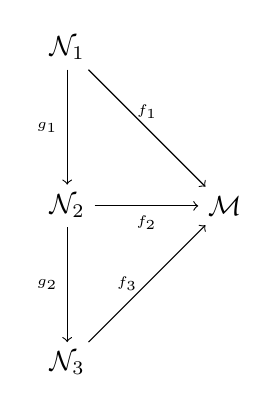
\begin{tikzpicture}[every path/.style={->}]
        \node (N1) at (0,0) {$\mathcal{N}_{1}$};
        \node (N2) at (0,-2) {$\mathcal{N}_{2}$};
        \node (N3) at (0,-4) {$\mathcal{N}_{3}$};
        \node (M) at (2,-2) {$\mathcal{M}$};
        \path (N1) edge node [above] {\tiny{$f_{1}$}} (M);
        \path (N2) edge node [below] {\tiny{$f_{2}$}} (M);
        \path (N3) edge node [left] {\tiny{$f_{3}$}} (M);
        \path (N1) edge node [left] {\tiny{$g_{1}$}} (N2);
        \path (N2) edge node [left] {\tiny{$g_{2}$}} (N3);
    \end{tikzpicture}
\end{document}